\documentclass[11pt]{l3deliverable}
\usepackage{geometry}
\usepackage{fullpage}
\usepackage{graphicx}
\usepackage{tabularx}
\usepackage{hyperref}
\usepackage{xcolor}
\definecolor{medium-red}{rgb}{0.35,0,0}
\hypersetup{colorlinks, linkcolor={medium-red}, citecolor={medium-red},
urlcolor={medium-red}}
\newcolumntype{T}{>{\centering\arraybackslash}m{0.20\textwidth}}
\newcolumntype{L}{>{\centering\arraybackslash}m{0.74\textwidth}}
\geometry{a4paper}
\setlength\parindent{0pt}
\title{System Design \& Acceptance Test Plan}
\deliverableID{D6}
\project{PSD3 Group Exercise 2}
\team{W}
\author{
    Gordon Reid: 1002536R\\
    Ryan Wells: 1002253W\\
    Kristopher Stewart: 1007175S\\
    David Selkirk: 1003646S\\
    James Gallagher: 0800899G\\
}
\date{\today}
\version{Final}
\begin{document}

\maketitle

\newpage

\tableofcontents

\newpage

\section{Introduction}

\subsection{Identification}

This is the design document and test plan for the internship management system
being developed by Team W for the Professional Software Engineering 3 course.
The internship management system is for Software Engineering (SE) and Electronic
and Software Engineering (ESE) students, studying in the school of Computing
Science.

\subsection{Related Documentation}

PSD3 Group Exercise Description:

\url{http://fims.moodle.gla.ac.uk/file.php/128/coursework/psd3-ge-2.pdf}

PSD3 Requirements Specification:

\url{http://fims.moodle.gla.ac.uk/file.php/128/coursework/requirements-specification-ge2.pdf}

PSD3 Forum Information:

\url{http://http://fims.moodle.gla.ac.uk/mod/forum/view.php?id=20433}

\subsection{Purpose and Description Of Document}

This document serves as the design document containing the overall system
architecture diagram with associated state charts. Each component in the
system architecture also has its own class diagrams and API specifications
specified.

The latter section of the document contains the acceptance test plan for
the implementation of the Internship Management System.

\subsection{Document Status and Schedule}

This document is the draft version of the deliverable and is subject to major
change.

Change log:

\begin{enumerate}
\item Updated title page to be consistent with other deliverables.
\item Updated introduction section to include requirements specification document
link and states that the document contains the acceptance test plan.
\item Updated system architecture diagram based on feedback.
\item Updated class diagrams and state diagrams.
\item Updated API specification.
\item Updated acceptance test plan to reflect actual test plan.
\item Updated with respect to forum information.
\end{enumerate}

\newpage

\section{System Architecture}

\subsection{Diagram}

\begin{centering}
  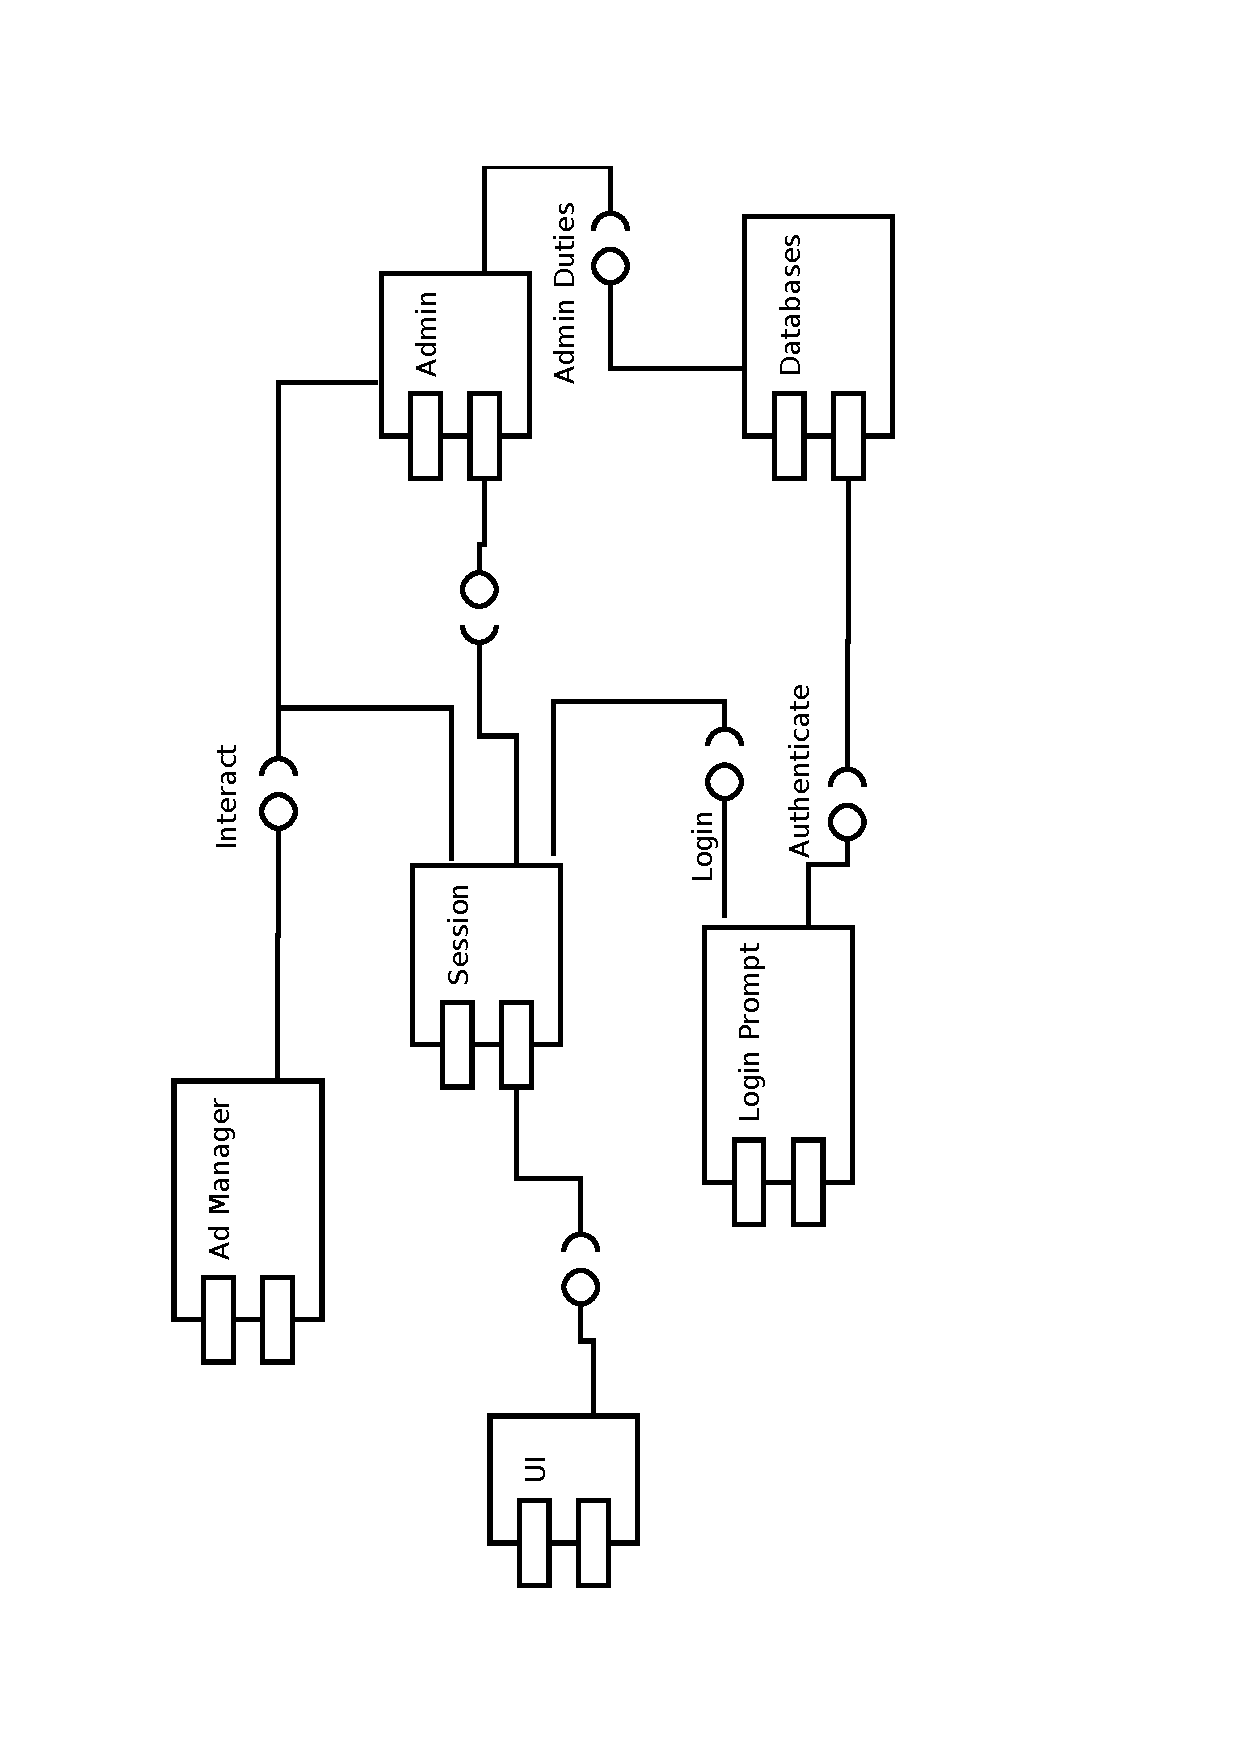
\includegraphics[width=\textwidth]{PSDDiagram.pdf}
\end{centering}

\subsection{Rationale}

We decided upon this system architecture as any component of the system should 
have the properties of being interchangeable with another substitutable 
component (substitutable defined as being having the same API). For this reason, 
we grouped related functionalities together and made them into a component. 
The `Ad Manager' and the `Databases' components could be combined together 
into one large `Database' component, but we did not want to create a coupling 
between these components - the `Ad Manager' may well have a database inside 
it, but the information inside this database is managed in a different way from 
the other data in the system such as users and companies.

All other components are defined by the primary reason that any component in the 
system can be replaced with no effect to the overall working of the system.

The `Session' component is essentially acting as a broker to user requests. This
simplifies the user interface's access to the functionality of the system and
further aids the ability for components to be swapped out with others as only
one component, the `Session' may have to be modified.

\newpage

\section{State Charts}

\subsection{Advertisement}

\subsubsection{Diagram}

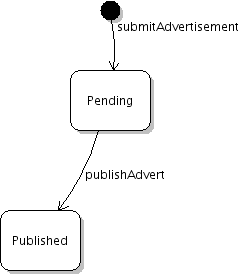
\includegraphics{advertState.png}

\subsubsection{Rationale}

The form of the state chart was decided based on the simplistic nature of an 
advertisements status. All adverts start off life as pending, after a company
has made the initial submission - however this is outside the scope of
the current system as it is not a ``must have'' use case. They can be
revised at any time prior to either being declined by the course
coordinator, where they are removed from the system and feedback sent
to the company(outside the scope) or published for viewing.

\subsection{Student}

\subsubsection{Diagram}

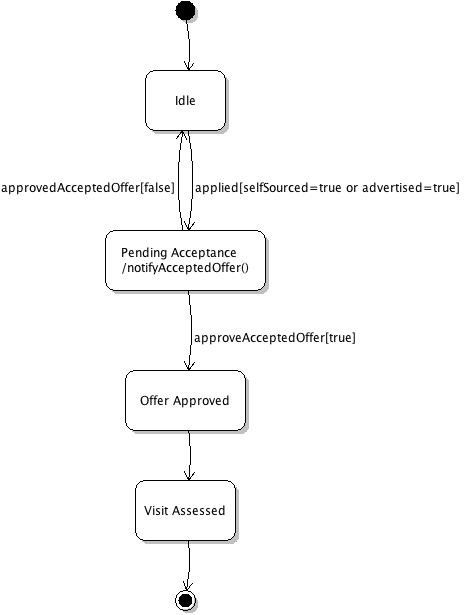
\includegraphics[width=0.9\textwidth]{studentState.png}

\subsubsection{Rationale}

We decided to create a state chart for a Student's flow through the
system as to clarify the functionality of the system with relation to
the student, and also for a base reason of a student having a
different state at multiple points in the system. There is one main
state that a student can take through this system to result in the
final state, this is modelling the best case scenario for a student
where a student will eventually end up with an approved final
placement, which we have interpreted as being one of the main
functionalities of the system. 

A student continually changes state between `Idle' and `Pending
Acceptance' (through either `Applied for Position' or `Found Self
Sourced Role') potentially multiple times until a suitable position
has been found and only then they will progress on to `Offer
Approved' which is the final resting state of this entity.

\newpage

\section{Class Diagrams and API Specifications}

\subsection{Advert Manager}

\subsubsection{Class Diagram}

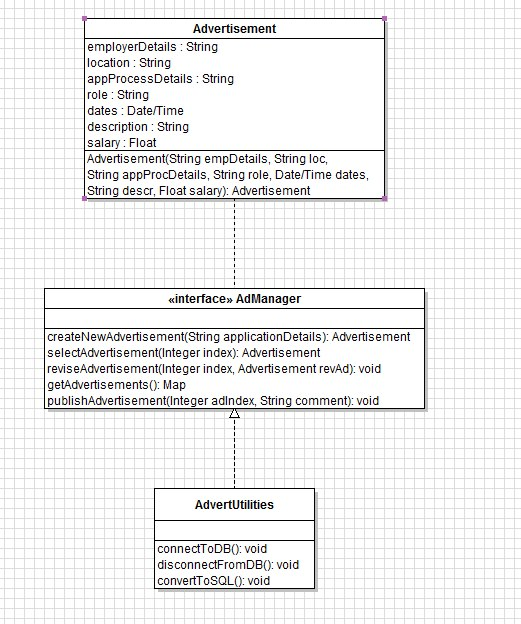
\includegraphics[width=\textwidth]{adManagerClassDiagram.png}

\subsubsection{API Specification}

\textbf{Full name}: public abstract interface AdManager\\

\textbf{Package}: uk.ac.glasgow.internman.AdManager

Each of the 3 available user types will be able to interact with this interface
but if the user has course coordinator rights then all available adverts can be
manipulated (published, denied etc), if they have registered employer rights
they'll be able to create/append and submit adverts for review and if they are
of type student, they'll only be able to view all published adverts.

\textbf{Methods}

\begin{itemize}

\item{\textbf{public Advertisement createNewAdvertisement(Employer e,
      String applicationDetails)}

Create a new advert with the specified details

\textbf{Preconditions:} User must be of type Course Coordinator or Employer

\textbf{Postconditions:} Advert is created and appended to a list of adverts awaiting 
review within the database.}

\item{\textbf{public Advertisement selectAdvertisement(Integer index)}

Given an index, select and display the appropriate advert from the database.

\textbf{Preconditions:} Must be a valid index

\textbf{Postconditions:} Advert is displayed after the index was successfully matched
in the database.}

\item{\textbf{public void reviseAdvertisement(Integer index, Advertisement revise)}

Using an index to select an existing advert, change its contents with that of another supplied.

\textbf{Preconditions:} Must be a valid index

\textbf{Postconditions:} Advert is successfully replaced with the revised one and the changes
can be seen dependant on its state, by others.}

\item{\textbf{public Map getAdvertisements()}

For use mostly by students who wish to see all available published adverts.

\textbf{Preconditions:} Must be at least one published advert

\textbf{Postconditions:} Advert(s) are displayed one after another in the UI with their
descriptions displayed.}

\item{\textbf{public void publishAdvertisement(Integer adIndex, String comment)}

Course coordinator only, select an advert and give feedback to the employer on why the advert was published.

\textbf{Preconditions:} Must be a valid index, comment must be supplied.

\textbf{Postconditions:} State of the selected advert is changed to published and can be
successfully viewed by students.}

\end{itemize}
\newpage

\subsection{Session}

\subsubsection{Class Diagram}

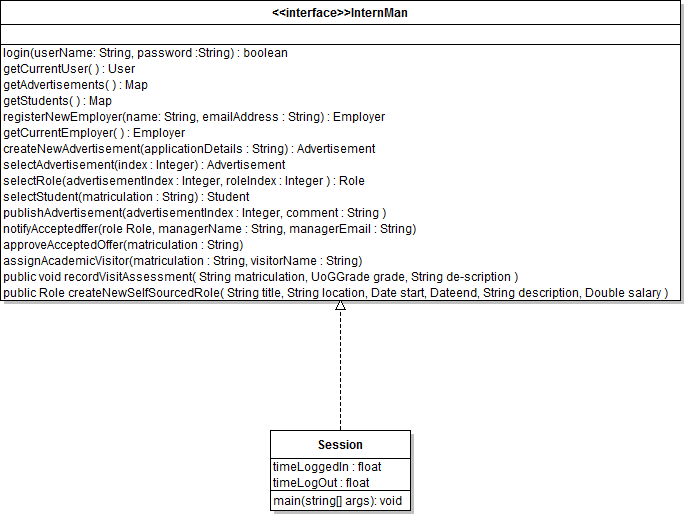
\includegraphics[scale=0.65,angle=90]{SessionClassDiagram.png}

\subsubsection{API Specification}

Session is purely the implementation of the supplied internship management
system API and doesn't supply functionality in its own right.

\newpage

\subsection{User Interface}

\subsubsection{Class Diagram}

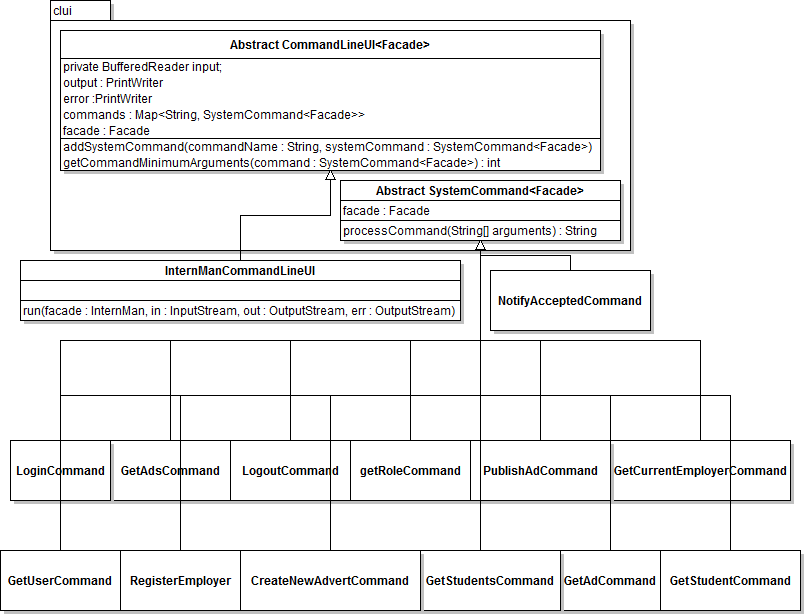
\includegraphics[scale=0.65,angle=90]{UIClassDiagram.png}

\subsubsection{API Specification}

\textbf{Full name:} public abstract interface InternManCommanLineUI\\

\textbf{Package:} uk.ac.glasgow.internman.ui\\

This is the interface for the graphical user interface.

\begin{itemize}

\item{\textbf{public void run(Facade facade, InputStream in, OutputStream out,
			OutputStream err)}

Runs the UI.

\textbf{Preconditions:} Facade must be constructed.

\textbf{Invariants:}

\textbf{Postconditions:} UI is displayed.}

\end{itemize}

\newpage

\subsection{Admin}

\subsubsection{Class Diagram}
\begin{centering}
  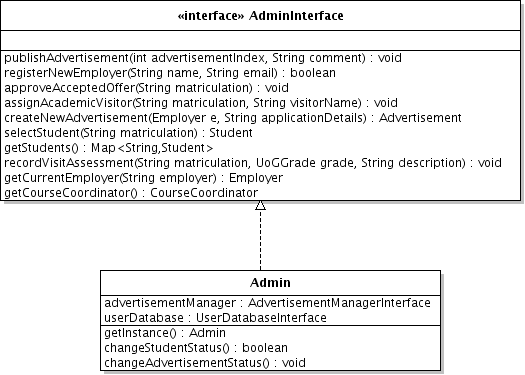
\includegraphics[width=0.7\textwidth]{adminClassDiagram.png}
\end{centering}
\subsubsection{API Specification}

\textbf{Full name:} public abstract interface Admin\\

\textbf{Package:} uk.ac.glasgow.internman.admin

This is the interface for the administration part of the database, accessible by
only the course coordinator.
This assumes that the user using this interface has Course Coordinator
rights.

\begin{itemize}

\item{\textbf{public void publishAdvertisement(Integer
    advertisementIndex, String comment)}

Approves an advertisement and makes it visible to students. Sends
comment as feedback to the employer as an email.

\textbf{Preconditions:} Advertisement must be in advertisement database.

\textbf{Invariants:}

\textbf{Postconditions:} Advertisement is now approved.}
%%%%%%%%%%%%%%%
\item{\textbf{public boolean registerNewEmployer(String name, String email)} 

Interface to add a company to the database, functionality is delegated to the
database component.
Error checking is done inside this function, but not whether or not a company
currently exists inside the companies database.

\textbf{Preconditions:} 

\textbf{Invariants:}

\textbf{Postconditions:} The return value of the delegated function indicates
the success of this function.}
%%%%%%%%%%%%%%%
\item{\textbf{public void approveAcceptedOffer(String matriculation)}

Approves the offer most recently accepted by the student with this matriculation
id. 
\textbf{Preconditions:} Student with this matriculation must have a successful
application and must have notified the Course Coordinator of their success.

\textbf{Invariants:} Student must not accept another successful application
during this review process.

\textbf{Postconditions:} Students status is changed to a success status.}
%%%%%%%%%%%%%%%
\item{\textbf{public void assignAcademicVisitor(String matriculation, String
    visitorName)}
Sends email to student, visitor and employer manager to let them know about
assignment. 

\textbf{Preconditions:} An academic visit cannot be currently assigned.

\textbf{Invariants:} 

\textbf{Postconditions:} }
%%%%%%%%%%%%%%%
\item{\textbf{public Advertisement createNewAdvertisement(Employer e,
      String applicationDetails)}
Adds a new (not-yet-approved) advertisement into the system.

\textbf{Preconditions:} Advertisement should not all ready exist in the
  system.

\textbf{Invariants:} 

\textbf{Postconditions:} }
%%%%%%%%%%%%%%%
\item{\textbf{public Student selectStudent( String matriculation)}
Gets handle on Student from supplied matriculation.

\textbf{Preconditions:} Null returned if Student is not in the map.

\textbf{Invariants:} 

\textbf{Postconditions:} }
%%%%%%%%%%%%%%%
\item{\textbf{public void recordVisitAssessment( String matriculation,
    UoGGrade grade, String description)}
Records grade for visit. Email to student and employer.

\textbf{Preconditions:} A visit assessment should not currently be
  assigned for this student

\textbf{Invariants:} 

\textbf{Postconditions:} }
%%%%%%%%%%%%%%
\item{\textbf{public Map<String,Student>getStudents()}
Returns a Mapping from matriculation to Student for every student in
the system.

\textbf{Preconditions:}

\textbf{Invariants:} 

\textbf{Postconditions:} }
%%%%%%%%%%%%%%
\item{\textbf{public Employer getCurrentEmployer( String employer )}
Selects the employer given by the String ``Employer''.

\textbf{Preconditions: Employer employer should exist within the
  system.}

\textbf{Invariants:} 

\textbf{Postconditions:} }
%%%%%%%%%%%%%%
\item{\textbf{public CourseCoordinator getCourseCoordinator() }
Gets the systems current Course Coordinator.

\textbf{Preconditions: }

\textbf{Invariants:} 

\textbf{Postconditions:} }


\end{itemize}

\subsection{Login Prompt}

\subsubsection{Class Diagram}

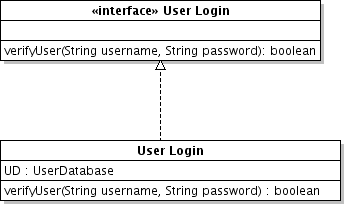
\includegraphics{loginClassDiagram.png}

\subsubsection{API Specification}

\textbf{Full name}: public abstract interface Login\\

\textbf{Package}: uk.ac.glasgow.internman.login

A user is presented with a prompt into which they must enter their MyCampus 
username and password. If the combination is valid, the user is logged in and 
presented with the summary of advertisements view.\\

\textbf{Methods}

\begin{itemize}

\item{\textbf{public Boolean verifyUser(String Id,String password)}

Check if a user is in database 

\textbf{Preconditions:} No user is currently logged in at the same user 
interface.}

\textbf{Invariants:}

\textbf{Postconditions:} User is logged in, if username and password combination 
is correct.
} 

\end{itemize}

\newpage

\subsection{Database}

\subsubsection{Class Diagram}

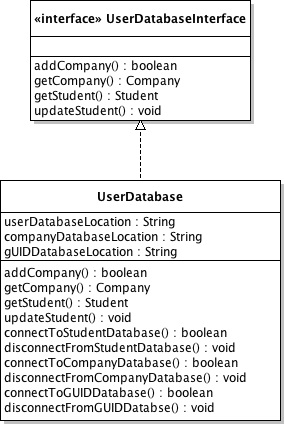
\includegraphics[width=\textwidth]{databaseClassDiagram.png}

\subsubsection{API Specification}

\textbf{Full name:} public abstract interface UserDatabase\\

\textbf{Package:} uk.ac.glasgow.internman.users

This is the interface for the user database. This database will hold information
on students, companies, and the course coordinator. For University students and
staff members, the database will access the MyCampus GUID system for login. For
companies, a separate store for their user information will be used.\\

\textbf{Methods}

\begin{itemize}

\item{\textbf{public boolean addEmployer(Employer e)}

Add information about an employer to the database.

\textbf{Preconditions:} Database must not already contain details of the 
employer.

\textbf{Invariants:}

\textbf{Postconditions:} Database now contains information about an employer 
including their login password.}

\item{\textbf{public Employer getEmployer(String username)}

Gets the employer with the given username.

\textbf{Preconditions:}

\textbf{Invariants:}

\textbf{Postconditions:} If a valid name is given, the object associated with
the company is returned, otherwise null is returned.}

\item{\textbf{public Map<String,Student> getStudents()}

Returns the mapping of String matriculation to Student's in the system.

\textbf{Preconditions:}

\textbf{Invariants:}

\textbf{Postconditions:}
}

\item{\textbf{public void updateStudent(Student student)}

Updates the user specific data for the supplied student. For example, when a
student obtains an internship, or has had their internship assessed.

\textbf{Preconditions:} Student must be a valid Computing Science student and
is known to the application's user database.

\textbf{Invariants:}

\textbf{Postconditions:} Student's user specific information is up to
date.}

\item{\textbf{public CourseCoordinator courseCoordinator()}

Returns the current course coordinator of the system.

\textbf{Preconditions:} 

\textbf{Invariants:}

\textbf{Postconditions:} If a course coordinator exists within the
system then they are returned (providing that the current user has
sufficient rights to do so) and if it does not then null is returned.}

\item{\textbf{public void changeCourseCoordinator(String username,
    String password)}
Changes the current Course Coordinators login details to the ones
supplied by the arguments username and password.

\textbf{Preconditions:}

\textbf{Invariants:}

\textbf{Postconditions:}}

\item{\textbf{public boolean loginStudent(String username, String
    password)} 
Returns whether or not the given username and password are valid
entries in the respective database.

\textbf{Preconditions:}

\textbf{Invariants:}

\textbf{Postconditions:}

}

\item{\textbf{public boolean loginEmployer(String username, String
    password)} 
Returns whether or not the given username and password are valid
entries in the respective database.

\textbf{Preconditions:}

\textbf{Invariants:}

\textbf{Postconditions:}

}

\item{\textbf{public boolean loginCourseCoordinator(String username, String
    password)} 
Returns whether or not the given username and password are valid
entries in the respective database.

\textbf{Preconditions:}

\textbf{Invariants:}

\textbf{Postconditions:}

}

\end{itemize}

\newpage

\begin{tabularx}{\textwidth}{|T|L|}
\hline
Identifier & UtilityAAO1\\
\hline
Use Case & Approve Accepted Offer \\
\hline
Description & Login as course coordinator and accept a student's internship.\\
\hline
Setup & A course coordinator and a student must be users in the system
before this test case is to be executed. If these users do not exist,
they must be added prior to execution. A successful application for
the referred student must also exist, and should be added and assigned
if it does not.\\
\hline
Interface & uk/ac/glasgow/internman \\
\hline
%%%%%%%%%%%%%%%%%%%%%%%%%%%%%%%%%%%%%%%%%%%%%%%%%%%%%%%%%%%%%%%%%%%%%%%%%%
Includes & Login \\
%%%%%%%%%%%%%%%%%%%%%%%%%%%%%%%%%%%%%%%%%%%%%%%%%%%%%%%%%%%%%%%%%%%%%%%%%%
\hline
Expected Outcome & Student now has their internship approved.\\
\hline
\end{tabularx}

\vspace{2em}

\begin{tabularx}{\textwidth}{|T|L|}
\hline
Identifier & UtilityAAO2\\
\hline
Use Case & Approve Accepted Offer \\
\hline
Description & Login as student and accept a student's internship.\\
\hline
Setup & A student with a successful application must exist in the
system. If this user does not exist, or if the successful application
does not exist then they should be created prior to execution. \\
\hline
Interface & uk/ac/glasgow/internman \\
\hline
Includes & UtilityTCLogin1 \\
\hline
Expected Outcome & Student 100000 has their internship still as ACCEPTED.\\
\hline
\end{tabularx}

\vspace{2em}

\begin{tabularx}{\textwidth}{|T|L|}
\hline
Identifier & UtilityAAO3\\
\hline
Use Case & Approve Accepted Offer \\
\hline
Description & Login as course coordinator and accept a student's internship.
The student does not exist.\\
\hline
Setup & A course coordinator should exist within the system. If this
user does not exist then it should be created prior to execution.
\hline
Interface & /uk/ac/glasgow/internman \\
\hline
%%%%%%%%%%%%%%%%%%%%%%%%%%%%%%%%%%%%%%%%%%%%%%%%%%%%%%%%%%%%%%%%%%%%%%%%%
Includes & Login \\
%%%%%%%%%%%%%%%%%%%%%%%%%%%%%%%%%%%%%%%%%%%%%%%%%%%%%%%%%%%%%%%%%%%%%%%%%
\hline
Expected Outcome & No change and program doesn't crash.\\
\hline
\end{tabularx}

\vspace{2em}

\begin{tabularx}{\textwidth}{|T|L|}
\hline
Identifier & UtilityTCLogin1\\
\hline
Use Case & Login\\
\hline
Description & Login a valid student. \\
\hline
Setup & A Student must exist in the system. If this user does not
exist in the system then it should be created prior to theo execution. \\
\hline
Interface & /uk/ac/glasgow/internman \\
\hline
Includes & \\
\hline
Expected Outcome & Student logged in, Student is now the current user
in the system.\\
\hline
\end{tabularx}

\vspace{2em}

\begin{tabularx}{\textwidth}{|T|L|}
\hline
Identifier & UtilityTCLogin2\\
\hline
Use Case & Login \\
\hline
Description & Login an invalid student. Valid username, invalid password\\
\hline
Setup & Student should exist in the system, if this is not the case
then this user should be created prior to execution.\\
\hline
Interface & /uk/ac/glasgow/internman \\
\hline
Includes & \\
\hline
Expected Outcome & Student not logged in, current user not changed.\\
\hline
\end{tabularx}

\vspace{2em}

\begin{tabularx}{\textwidth}{|T|L|}
\hline
Identifier & UtilityTCLogin3\\
\hline
Use Case & Login \\
\hline
Description & Login an invalid student. Invalid username\\
\hline
Setup & No setup required.\\
\hline
Interface & /uk/ac/glasgow/internman \\
\hline
Includes & \\
\hline
Expected Outcome & Student not logged in, current user not changed.\\
\hline
\end{tabularx}

\vspace{2em}

\begin{tabularx}{\textwidth}{|T|L|}
\hline
Identifier & UtilityTCLogin4\\
\hline
Use Case & Login \\
\hline
Description & Login a valid employer. \\
\hline
Setup & Employer should exist in the system, if this is not the case
then this user should be created prior to execution. \\
\hline
Interface & /uk/ac/glasgow/internman \\
\hline
Includes & \\
\hline
Expected Outcome & Employer  logged in, Employer is set as current
user in the system. \\
\hline
\end{tabularx}

\vspace{2em}

\begin{tabularx}{\textwidth}{|T|L|}
\hline
Identifier & UtilityTCLogin5\\
\hline
Use Case & Login \\
\hline
Description & Login an invalid employer. Valid username, invalid password\\
\hline
Setup & Employer should exist in the system, if this is not the case
then this user should be created prior to execution. \\
\hline
Interface & /uk/ac/glasgow/internman \\
\hline
Includes & \\
\hline
Expected Outcome & Employer not logged in, current user is not
changed.\\
\hline
\end{tabularx}

\vspace{2em}

\begin{tabularx}{\textwidth}{|T|L|}
\hline
Identifier & UtilityTCLogin6\\
\hline
Use Case & Login \\
\hline
Description & Login an invalid employer. Invalid username. \\
\hline
Setup & No setup required. \\
\hline
Interface & /uk/ac/glasgow/internman \\
\hline
Includes & \\
\hline
Expected Outcome & Employer not logged in, current user is not
changed.\\
\hline
\end{tabularx}

\vspace{2em}

\begin{tabularx}{\textwidth}{|T|L|}
\hline
Identifier & UtilityTCLogin7\\
\hline
Use Case & Login \\
\hline
Description & Login a valid course coordinator. \\
\hline
Setup & Course Coordinator must exist inside the system, if this is
not the case then this user should be created prior to execution. \\
\hline
Interface & /uk/ac/glasgow/internman \\
\hline
Includes & \\
\hline
Expected Outcome & Course coordinator logged in, Course
Coordinator is now current user.\\
\hline
\end{tabularx}

\vspace{2em}

\begin{tabularx}{\textwidth}{|T|L|}
\hline
Identifier & UtilityTCLogin8\\
\hline
Use Case & Login \\
\hline
Description & Login an invalid course coordinator. Valid username,
invalid password. \\
\hline
Setup & Course Coordinator must exist inside the system, if this is
not the case then this user should be created prior to execution. \\
\hline
Interface & /uk/ac/glasgow/internman \\
\hline
Includes & \\
\hline
Expected Outcome & Course coordinator not logged in, current user is
not changed. \\
\hline
\end{tabularx}

\vspace{2em}

\begin{tabularx}{\textwidth}{|T|L|}
\hline
Identifier & UtilityTCLogin9\\
\hline
Use Case & Login \\
\hline
Description & Login an invalid course coordinator. Invalid username.\\
\hline
Setup & No setup required. \\
\hline
Interface & /uk/ac/glasgow/internman \\
\hline
Includes & \\
\hline
Expected Outcome & Course coordinator not logged in, current user is
not changed. \\
\hline
\end{tabularx}

\begin{tabularx}{\textwidth}{|T|L|}
\hline
Identifier & UtilityNAO1\\
\hline
Use Case & Notify Accepted Offer \\
\hline
Description & Login as course coordinator and notify course
coordinator of an internship.\\
\hline
Setup & Course coordinator should exist within the system and an
internship should also exist within the system. If these entities do
not exist then they should be created prior to execution.\\
\hline
Interface & /uk/ac/glasgow/internman \\
\hline
Includes & \\
\hline
Expected Outcome & Attempt should fail, course coordinators do not do
internships.\\
\hline
\end{tabularx}

\vspace{2em}

\begin{tabularx}{\textwidth}{|T|L|}
\hline
Identifier & UtilityNAO2\\
\hline
Date Tested & 18/02/2013\\
\hline
Tester & Gordon Reid - 1002536r\\
\hline
Description & Login as an employer and notify course coordinator of an 
internship.\\
\hline
Setup & None possible - unable to add own users or modify them.\\
\hline
Pass/Fail & \cellcolor{red}Fail\\
\hline
Expected Outcome & Nothing, employers do not do internships.\\
\hline
Actual Outcome & Null pointer exception.\\
\hline
Additional Comments & Due to login failure and the facade assumption that a
user is logged in, null pointer exception happens.\\
\hline
\end{tabularx}

\vspace{2em}

\begin{tabularx}{\textwidth}{|T|L|}
\hline
Identifier & UtilityNAO3\\
\hline
Date Tested & 18/02/2013\\
\hline
Tester & Gordon Reid - 1002536r\\
\hline
Description & Login as course coordinator and accept a student's internship.
The student does not exist.\\
\hline
Setup & None possible - unable to add own users or modify them.\\
\hline
Pass/Fail & \cellcolor{red}Fail\\
\hline
Expected Outcome & No change and program doesn't crash.\\
\hline
Actual Outcome & Null pointer exception.\\
\hline
Additional Comments & Due to login failure and the facade assumption that a
user is logged in, null pointer exception happens.\\
\hline
\end{tabularx}

\begin{tabularx}{\textwidth}{|T|L|}
\hline
Identifier & UtilityPA1\\
\hline
Date Tested & 18/02/2013\\
\hline
Tester & Gordon Reid - 1002536r\\
\hline
Description & Login as course coordinator publish an advertisement so a 
student can view it.\\
\hline
Setup & None possible - unable to add own users or modify them.\\
\hline
Pass/Fail & \cellcolor{red}Fail\\
\hline
Expected Outcome & Advertisement is published and available to be viewed by
a student.\\
\hline
Actual Outcome & Null pointer exception.\\
\hline
Additional Comments & Due to login failure and the facade assumption that a user 
is logged in, null pointer exception happens.\\
\hline
\end{tabularx}

\vspace{2em}

\begin{tabularx}{\textwidth}{|T|L|}
\hline
Identifier & UtilityPA2\\
\hline
Date Tested & 18/02/2013\\
\hline
Tester & Gordon Reid - 1002536r\\
\hline
Description & Login as course coordinator publish an advertisement and still
have the course coordinator view it.\\
\hline
Setup & None possible - unable to add own users or modify them.\\
\hline
Pass/Fail & \cellcolor{red}Fail\\
\hline
Expected Outcome & Advertisement is published and available to be viewed by the
course coordinator.\\
\hline
Actual Outcome & Null pointer exception.\\
\hline
Additional Comments & Due to login failure and the facade assumption that a user 
is logged in, null pointer exception happens.\\
\hline
\end{tabularx}

\vspace{2em}

\begin{tabularx}{\textwidth}{|T|L|}
\hline
Identifier & UtilityPA3\\
\hline
Date Tested & 18/02/2013\\
\hline
Tester & Gordon Reid - 1002536r\\
\hline
Description & Login as course coordinator publish an advertisement and still
have the employer who created it view it.\\
\hline
Setup & None possible - unable to add own users or modify them.\\
\hline
Pass/Fail & \cellcolor{red}Fail\\
\hline
Expected Outcome & Advertisement is published and available to be viewed by the
owner employer.\\
\hline
Actual Outcome & Null pointer exception.\\
\hline
Additional Comments & Due to login failure and the facade assumption that a user 
is logged in, null pointer exception happens.\\
\hline
\end{tabularx}

\vspace{2em}

\begin{tabularx}{\textwidth}{|T|L|}
\hline
Identifier & UtilityPA4\\
\hline
Date Tested & 18/02/2013\\
\hline
Tester & Gordon Reid - 1002536r\\
\hline
Description & Login as course coordinator publish an advertisement that
doesn't exist, then try to get a student to view it.\\
\hline
Setup & None possible - unable to add own users or modify them.\\
\hline
Pass/Fail & \cellcolor{red}Fail\\
\hline
Expected Outcome & Nothing happens as advert doesn't exist.\\
\hline
Actual Outcome & Null pointer exception.\\
\hline
Additional Comments & The facade assumes that an advertisement exists so
null pointer exception happens.\\
\hline
\end{tabularx}

\vspace{2em}

\begin{tabularx}{\textwidth}{|T|L|}
\hline
Identifier & UtilityPA5\\
\hline
Date Tested & 18/02/2013\\
\hline
Tester & Gordon Reid - 1002536r\\
\hline
Description & Login as course coordinator publish an advertisement that
doesn't exist, then try to get the course coordinator to view it.\\
\hline
Setup & None possible - unable to add own users or modify them.\\
\hline
Pass/Fail & \cellcolor{red}Fail\\
\hline
Expected Outcome & Nothing happens as advert doesn't exist.\\
\hline
Actual Outcome & Null pointer exception.\\
\hline
Additional Comments & The facade assumes that an advertisement exists so
null pointer exception happens.\\
\hline
\end{tabularx}

\vspace{2em}

\begin{tabularx}{\textwidth}{|T|L|}
\hline
Identifier & UtilityPA6\\
\hline
Date Tested & 18/02/2013\\
\hline
Tester & Gordon Reid - 1002536r\\
\hline
Description & Login as course coordinator publish an advertisement that
doesn't exist, then try to get an employer to view it.\\
\hline
Setup & None possible - unable to add own users or modify them.\\
\hline
Pass/Fail & \cellcolor{red}Fail\\
\hline
Expected Outcome & Nothing happens as advert doesn't exist.\\
\hline
Actual Outcome & Null pointer exception.\\
\hline
Additional Comments & The facade assumes that an advertisement exists so
null pointer exception happens.\\
\hline
\end{tabularx}

\begin{tabularx}{\textwidth}{|T|L|}
\hline
Identifier & UtilityRE1\\
\hline
Date Tested & 18/02/2013\\
\hline
Tester & Gordon Reid - 1002536r\\
\hline
Description & Login as course coordinator and add a new employer.\\
\hline
Setup & None possible - unable to add own users or modify them.\\
\hline
Pass/Fail & \cellcolor{green}Pass\\
\hline
Expected Outcome & New employer added to the database.\\
\hline
Actual Outcome & New employer added to the database.\\
\hline
Additional Comments &\\
\hline
\end{tabularx}

\vspace{2em}

\begin{tabularx}{\textwidth}{|T|L|}
\hline
Identifier & UtilityRE2\\
\hline
Date Tested & 18/02/2013\\
\hline
Tester & Gordon Reid - 1002536r\\
\hline
Description & Login as student and add a new employer.\\
\hline
Setup & None possible - unable to add own users or modify them.\\
\hline
Pass/Fail & \cellcolor{red}Fail\\
\hline
Expected Outcome & Nothing, student cannot add employers.\\
\hline
Actual Outcome & Null pointer exception.\\
\hline
Additional Comments & Due to login failure and the facade assumption that a user 
is logged in, null pointer exception happens.\\
\hline
\end{tabularx}

\vspace{2em}

\begin{tabularx}{\textwidth}{|T|L|}
\hline
Identifier & UtilityRE3\\
\hline
Date Tested & 18/02/2013\\
\hline
Tester & Gordon Reid - 1002536r\\
\hline
Description & Login as employer and add a new employer.\\
\hline
Setup & None possible - unable to add own users or modify them.\\
\hline
Pass/Fail & \cellcolor{red}Fail\\
\hline
Expected Outcome & Nothing, employers cannot add employers.\\
\hline
Actual Outcome & Null pointer exception.\\
\hline
Additional Comments & Due to login failure and the facade assumption that a user 
is logged in, null pointer exception happens.\\
\hline
\end{tabularx}

\vspace{2em}


\begin{tabularx}{\textwidth}{|T|L|}
\hline
Identifier & UtilitySA1\\
\hline
Date Tested & 18/02/2013\\
\hline
Tester & Gordon Reid - 1002536r\\
\hline
Description & Login as employer and submit an advertisement.\\
\hline
Setup & None possible - unable to add own users or modify them.\\
\hline
Pass/Fail & \cellcolor{red}Fail\\
\hline
Expected Outcome & New advertisement to be published added to the database.\\
\hline
Actual Outcome & Null pointer exception.\\
\hline
Additional Comments & Due to login failure and the facade assumption that a user 
is logged in, null pointer exception happens.\\
\hline
\end{tabularx}

\vspace{2em}

\begin{tabularx}{\textwidth}{|T|L|}
\hline
Identifier & UtilitySA2\\
\hline
Date Tested & 18/02/2013\\
\hline
Tester & Gordon Reid - 1002536r\\
\hline
Description & Login as course coordinator and submit an advertisement.\\
\hline
Setup & None possible - unable to add own users or modify them.\\
\hline
Pass/Fail & \cellcolor{green}Pass\\
\hline
Expected Outcome & New advertisement to be published added to the database.\\
\hline
Actual Outcome & New advertisement to be published added to the database.\\
\hline
Additional Comments &\\
\hline
\end{tabularx}

\vspace{2em}

\begin{tabularx}{\textwidth}{|T|L|}
\hline
Identifier & UtilitySA3\\
\hline
Date Tested & 18/02/2013\\
\hline
Tester & Gordon Reid - 1002536r\\
\hline
Description & Login as student and submit an advertisement.\\
\hline
Setup & None possible - unable to add own users or modify them.\\
\hline
Pass/Fail & \cellcolor{red}Fail\\
\hline
Expected Outcome & Nothing, students cannot submit advertisements.\\
\hline
Actual Outcome & Null pointer exception.\\
\hline
Additional Comments & Due to login failure and the facade assumption that a user 
is logged in, null pointer exception happens.\\
\hline
\end{tabularx}

\vspace{2em}

\begin{tabularx}{\textwidth}{|T|L|}
\hline
Identifier & UtilitySA4\\
\hline
Date Tested & 18/02/2013\\
\hline
Tester & Gordon Reid - 1002536r\\
\hline
Description & Don't login and submit an advertisement.\\
\hline
Setup & None possible - unable to add own users or modify them.\\
\hline
Pass/Fail & \cellcolor{red}Fail\\
\hline
Expected Outcome & Nothing, you need to login to submit advertisements.\\
\hline
Actual Outcome & Null pointer exception.\\
\hline
Additional Comments & Due to the facade assumption that a user 
is logged in, null pointer exception happens.\\
\hline
\end{tabularx}

\begin{tabularx}{\textwidth}{|T|L|}
\hline
Identifier & UtilityVA1\\
\hline
Date Tested & 18/02/2013\\
\hline
Tester & Gordon Reid - 1002536r\\
\hline
Description & Login as student and view a published advertisement.\\
\hline
Setup & None possible - unable to add own users or modify them.\\
\hline
Pass/Fail & \cellcolor{red}Fail\\
\hline
Expected Outcome & Advertisement details available.\\
\hline
Actual Outcome & Null pointer exception.\\
\hline
Additional Comments & Advert creation and publication doesn't work causing
failure.\\
\hline
\end{tabularx}

\vspace{2em}

\begin{tabularx}{\textwidth}{|T|L|}
\hline
Identifier & UtilityVA2\\
\hline
Date Tested & 18/02/2013\\
\hline
Tester & Gordon Reid - 1002536r\\
\hline
Description & Login as course coordinator and view a published advertisement.\\
\hline
Setup & None possible - unable to add own users or modify them.\\
\hline
Pass/Fail & \cellcolor{red}Fail\\
\hline
Expected Outcome & Advertisement details available.\\
\hline
Actual Outcome & Null pointer exception.\\
\hline
Additional Comments & Advert creation and publication doesn't work causing
failure.\\
\hline
\end{tabularx}

\vspace{2em}

\begin{tabularx}{\textwidth}{|T|L|}
\hline
Identifier & UtilityVA3\\
\hline
Date Tested & 18/02/2013\\
\hline
Tester & Gordon Reid - 1002536r\\
\hline
Description & Login as owner company and view their published advertisement.\\
\hline
Setup & None possible - unable to add own users or modify them.\\
\hline
Pass/Fail & \cellcolor{red}Fail\\
\hline
Expected Outcome & Advertisement details available.\\
\hline
Actual Outcome & Null pointer exception.\\
\hline
Additional Comments & Advert creation and publication doesn't work causing
failure.\\
\hline
\end{tabularx}

\vspace{2em}

\begin{tabularx}{\textwidth}{|T|L|}
\hline
Identifier & UtilityVA4\\
\hline
Date Tested & 18/02/2013\\
\hline
Tester & Gordon Reid - 1002536r\\
\hline
Description & Login as an employer and view another employers published 
advertisement.\\
\hline
Setup & None possible - unable to add own users or modify them.\\
\hline
Pass/Fail & \cellcolor{red}Fail\\
\hline
Expected Outcome & Advertisement details unavailable.\\
\hline
Actual Outcome & Null pointer exception.\\
\hline
Additional Comments & Advert creation and publication doesn't work causing
failure.\\
\hline
\end{tabularx}

\vspace{2em}

\begin{tabularx}{\textwidth}{|T|L|}
\hline
Identifier & UtilityVA5\\
\hline
Date Tested & 18/02/2013\\
\hline
Tester & Gordon Reid - 1002536r\\
\hline
Description & Login as course coordinator and view a pending advertisement.\\
\hline
Setup & None possible - unable to add own users or modify them.\\
\hline
Pass/Fail & \cellcolor{red}Fail\\
\hline
Expected Outcome & Advertisement details available.\\
\hline
Actual Outcome & Null pointer exception.\\
\hline
Additional Comments & Advert creation and publication doesn't work causing
failure.\\
\hline
\end{tabularx}

\vspace{2em}

\begin{tabularx}{\textwidth}{|T|L|}
\hline
Identifier & UtilityVA6\\
\hline
Date Tested & 18/02/2013\\
\hline
Tester & Gordon Reid - 1002536r\\
\hline
Description & Login as student and view a pending advertisement.\\
\hline
Setup & None possible - unable to add own users or modify them.\\
\hline
Pass/Fail & \cellcolor{red}Fail\\
\hline
Expected Outcome & Advertisement details unavailable.\\
\hline
Actual Outcome & Null pointer exception.\\
\hline
Additional Comments & Advert creation and publication doesn't work causing
failure.\\
\hline
\end{tabularx}

\vspace{2em}

\begin{tabularx}{\textwidth}{|T|L|}
\hline
Identifier & UtilityVA7\\
\hline
Date Tested & 18/02/2013\\
\hline
Tester & Gordon Reid - 1002536r\\
\hline
Description & Login as owner company and view their pending advertisement.\\
\hline
Setup & None possible - unable to add own users or modify them.\\
\hline
Pass/Fail & \cellcolor{red}Fail\\
\hline
Expected Outcome & Advertisement details available.\\
\hline
Actual Outcome & Null pointer exception.\\
\hline
Additional Comments & Advert creation and publication doesn't work causing
failure.\\
\hline
\end{tabularx}

\vspace{2em}

\begin{tabularx}{\textwidth}{|T|L|}
\hline
Identifier & UtilityVA8\\
\hline
Date Tested & 18/02/2013\\
\hline
Tester & Gordon Reid - 1002536r\\
\hline
Description & Login as some employer and view another's pending advertisement.\\
\hline
Setup & None possible - unable to add own users or modify them.\\
\hline
Pass/Fail & \cellcolor{red}Fail\\
\hline
Expected Outcome & Advertisement details available.\\
\hline
Actual Outcome & Null pointer exception.\\
\hline
Additional Comments & Advert creation and publication doesn't work causing
failure.\\
\hline
\end{tabularx}


\begin{tabularx}{\textwidth}{|T|L|}
\hline
Identifier & UtilityVS1\\
\hline
Date Tested & 18/02/2013\\
\hline
Tester & Gordon Reid - 1002536r\\
\hline
Description & Login as course coordinator and view a student.\\
\hline
Setup & None possible - unable to add own users or modify them.\\
\hline
Pass/Fail & \cellcolor{red}Fail\\
\hline
Expected Outcome & Student details available.\\
\hline
Actual Outcome & Null pointer exception.\\
\hline
Additional Comments & No students exist in system and none can be added.\\
\hline
\end{tabularx}

\vspace{2em}

\begin{tabularx}{\textwidth}{|T|L|}
\hline
Identifier & UtilityVS2\\
\hline
Date Tested & 18/02/2013\\
\hline
Tester & Gordon Reid - 1002536r\\
\hline
Description & Login as course coordinator and view a nonexistent student.\\
\hline
Setup & None possible - unable to add own users or modify them.\\
\hline
Pass/Fail & \cellcolor{green}Pass\\
\hline
Expected Outcome & Nothing, student doesn't exist.\\
\hline
Actual Outcome & Nothing, student doesn't exist.\\
\hline
Additional Comments & No students exist in system and none can be added.\\
\hline
\end{tabularx}

\vspace{2em}

\begin{tabularx}{\textwidth}{|T|L|}
\hline
Identifier & UtilityVS3\\
\hline
Date Tested & 18/02/2013\\
\hline
Tester & Gordon Reid - 1002536r\\
\hline
Description & Login as employer and view a student.\\
\hline
Setup & None possible - unable to add own users or modify them.\\
\hline
Pass/Fail & \cellcolor{red}Fail\\
\hline
Expected Outcome & Student details unavailable, employers cannot view
students.\\
\hline
Actual Outcome & Null pointer exception.\\
\hline
Additional Comments & No students exist in system and none can be added.\\
\hline
\end{tabularx}

\vspace{2em}
\begin{tabularx}{\textwidth}{|T|L|}
\hline
Identifier & UtilityVS4\\
\hline
Date Tested & 18/02/2013\\
\hline
Tester & Gordon Reid - 1002536r\\
\hline
Description & Login as student and view a student.\\
\hline
Setup & None possible - unable to add own users or modify them.\\
\hline
Pass/Fail & \cellcolor{red}Fail\\
\hline
Expected Outcome & Student details unavailable, students cannot view
students.\\
\hline
Actual Outcome & Null pointer exception.\\
\hline
Additional Comments & No students exist in system and none can be added.\\
\hline
\end{tabularx}

\vspace{2em}


\end{document}
